\documentclass[10pt]{article}
\usepackage[T1]{fontenc}
\usepackage{lmodern,amsmath,amssymb,booktabs,array,graphicx,tikz,pgfplots}
\usepackage[paperwidth=190mm,paperheight=224mm,margin=10mm]{geometry}
\usepackage[hidelinks]{hyperref}
\hypersetup{pdfauthor={},pdftitle={Monochrome mathematical illustrations: semiconductor-health identifiability}}
\usetikzlibrary{arrows.meta,positioning,calc,patterns}
\pgfplotsset{compat=1.18}
\newcommand{\trans}{^{\mathsf T}}\newcommand{\R}{\mathbb R}
\newcommand{\one}{\mathbf 1}\newcommand{\zero}{\mathbf 0}
\DeclareMathOperator{\rank}{rank}\DeclareMathOperator{\range}{range}
\DeclareMathOperator{\diag}{diag}\DeclareMathOperator{\Cov}{Cov}
\DeclareMathOperator{\Var}{Var}\DeclareMathOperator{\spanop}{span}
\newcommand{\FigureNote}{Visualization code prepared with assistance from OpenAI Codex.}
\pagestyle{empty}\setlength{\parindent}{0pt}
\tikzset{
 every picture/.style={font=\fontsize{9}{11}\selectfont,>=Latex},
 every node/.style={font=\fontsize{9}{11}\selectfont,inner sep=2pt},
 head/.style={font=\fontsize{9.5}{12}\selectfont\bfseries,anchor=west},
 tinytext/.style={font=\fontsize{8}{10}\selectfont},eq/.style={align=center},
 wire/.style={draw=black,line width=.5pt},arr/.style={->,black,line width=.65pt},
 device/.style={draw,fill=white,minimum width=1.1cm,minimum height=.38cm}}
\pgfplotsset{mathaxis/.style={axis lines=left,axis line style={black,line width=.5pt},
 tick style={black},tick label style={font=\fontsize{8}{10}\selectfont},
 label style={font=\fontsize{8.5}{10}\selectfont},grid=major,
 major grid style={black!15,line width=.2pt},
 legend style={font=\fontsize{8}{10}\selectfont,draw=none,fill=white},
 every axis plot/.append style={black}}}
\newcommand{\PlateTitle}[2]{\small\textbf{Mathematical plate #1}\hfill Monochrome TikZ / PGFPlots\par
 \vspace{1.5mm}{\large\bfseries #2}\par\vspace{2mm}}
\newcommand{\PlateCaption}[1]{\par\vspace{1mm}{\fontsize{8.5}{10.5}\selectfont #1\par
 \vspace{1mm}\FigureNote\par}}

\begin{document}
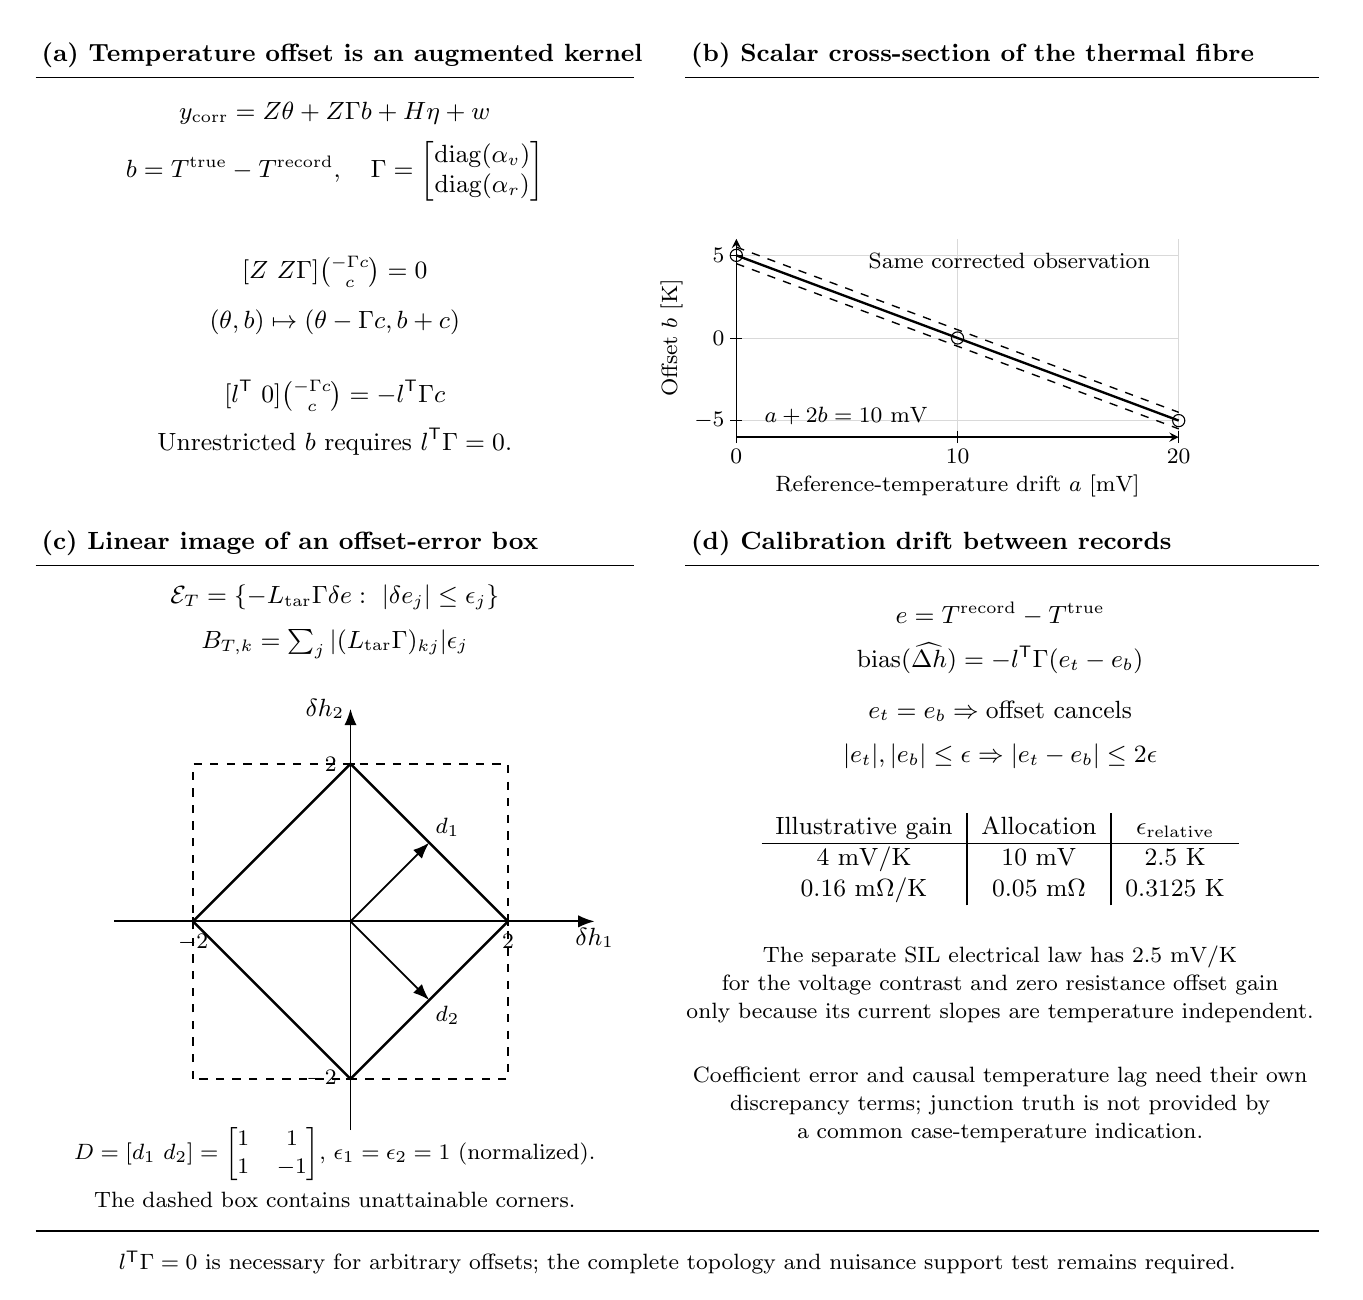
\begin{tikzpicture}[x=1cm,y=1cm]\path[use as bounding box] (0,0) rectangle (16.6,15.8);
\node[head] at (0.1,15.45){(a) Temperature offset is an augmented kernel};\draw[wire] (0.1,15.17)--(7.699999999999999,15.17);
\node[head] at (8.35,15.45){(b) Scalar cross-section of the thermal fibre};\draw[wire] (8.35,15.17)--(16.4,15.17);
\node[eq] at (3.9,14.22){$y_{\mathrm{corr}}=Z\theta+Z\Gamma b+H\eta+w$\\[5pt]
$b=T^{\mathrm{true}}-T^{\mathrm{record}},\quad\Gamma=\begin{bmatrix}\diag(\alpha_v)\\\diag(\alpha_r)\end{bmatrix}$};
\node[eq] at (3.9,12.4){$[Z\ Z\Gamma]\binom{-\Gamma c}{c}=0$\\[7pt]$(\theta,b)\mapsto(\theta-\Gamma c,b+c)$};
\node[eq] at (3.9,10.85){$[l\trans\ 0]\binom{-\Gamma c}{c}=-l\trans\Gamma c$\\[5pt]Unrestricted $b$ requires $l\trans\Gamma=0$.};
\begin{axis}[mathaxis,at={(9.0cm,10.6cm)},anchor=south west,width=7.2cm,height=4.1cm,
 xmin=0,xmax=20,ymin=-6,ymax=6,xtick={0,10,20},ytick={-5,0,5},
 xlabel={Reference-temperature drift $a$ [mV]},ylabel={Offset $b$ [K]},clip=false]
\addplot[domain=0:20,samples=2,line width=.85pt]{(10-x)/2};
\addplot[domain=0:20,samples=2,dashed,line width=.5pt]{(11-x)/2};
\addplot[domain=0:20,samples=2,dashed,line width=.5pt]{(9-x)/2};
\addplot[only marks,mark=o,mark size=2.2pt] coordinates {(0,5)(10,0)(20,-5)};
\node[tinytext,anchor=west] at (axis cs:1,-4.7){$a+2b=10$ mV};
\node[tinytext,anchor=east] at (axis cs:19,4.7){Same corrected observation};\end{axis}
\node[head] at (0.1,9.25){(c) Linear image of an offset-error box};\draw[wire] (0.1,8.97)--(7.699999999999999,8.97);
\node[head] at (8.35,9.25){(d) Calibration drift between records};\draw[wire] (8.35,8.97)--(16.4,8.97);
\node[eq] at (3.9,8.25){$\mathcal E_T=\{-L_{\mathrm{tar}}\Gamma\delta e:\ |\delta e_j|\leq\epsilon_j\}$\\[5pt]
$B_{T,k}=\sum_j |(L_{\mathrm{tar}}\Gamma)_{kj}|\epsilon_j$};
\draw[arr] (1.1,4.45)--(7.2,4.45) node[below] {$\delta h_1$};
\draw[arr] (4.1,1.8)--(4.1,7.15) node[left] {$\delta h_2$};
\draw[dashed,wire] (2.1,2.45) rectangle (6.1,6.45);
\draw[line width=.9pt] (2.1,4.45)--(4.1,6.45)--(6.1,4.45)--(4.1,2.45)--cycle;
\draw[arr] (4.1,4.45)--(5.1,5.45) node[above right,tinytext] {$d_1$};
\draw[arr] (4.1,4.45)--(5.1,3.45) node[below right,tinytext] {$d_2$};
\foreach \xx/\lab in {2.1/-2,6.1/2}{\draw[wire] (\xx,4.39)--(\xx,4.51);\node[tinytext,below] at (\xx,4.37){$\lab$};}
\foreach \yy/\lab in {2.45/-2,6.45/2}{\draw[wire] (4.04,\yy)--(4.16,\yy);\node[tinytext,left] at (4.0,\yy){$\lab$};}
\node[tinytext,align=center] at (3.9,1.5){$D=[d_1\ d_2]=\begin{bmatrix}1&1\\1&-1\end{bmatrix}$, $\epsilon_1=\epsilon_2=1$ (normalized).};
\node[tinytext] at (3.9,.92){The dashed box contains unattainable corners.};
\node[eq] at (12.35,8.05){$e=T^{\mathrm{record}}-T^{\mathrm{true}}$\\[5pt]$\operatorname{bias}(\widehat{\Delta h})=-l\trans\Gamma(e_t-e_b)$};
\node[eq] at (12.35,6.82){$e_t=e_b\Rightarrow\text{offset cancels}$\\[5pt]$|e_t|,|e_b|\leq\epsilon\Rightarrow|e_t-e_b|\leq2\epsilon$};
\node[eq] at (12.35,5.24){$\begin{array}{c|c|c}\text{Illustrative gain}&\text{Allocation}&\epsilon_{\mathrm{relative}}\\\hline
4\ \mathrm{mV/K}&10\ \mathrm{mV}&2.5\ \mathrm K\\0.16\ \mathrm{m}\Omega/\mathrm K&0.05\ \mathrm{m}\Omega&0.3125\ \mathrm K\end{array}$};
\node[tinytext,align=center] at (12.35,3.65){The separate SIL electrical law has 2.5 mV/K\\for the voltage contrast and zero resistance offset gain\\only because its current slopes are temperature independent.};
\node[tinytext,align=center] at (12.35,2.12){Coefficient error and causal temperature lag need their own\\discrepancy terms; junction truth is not provided by\\a common case-temperature indication.};
\draw[wire] (.1,.52)--(16.4,.52);
\node[tinytext] at (8.25,.12){$l\trans\Gamma=0$ is necessary for arbitrary offsets; the complete topology and nuisance support test remains required.};\end{tikzpicture}
\end{document}
